\documentclass{article}
\addtolength{\oddsidemargin}{-.875in}
\addtolength{\evensidemargin}{-.875in}
\addtolength{\textwidth}{1.75in}

\addtolength{\topmargin}{-.875in}
\addtolength{\textheight}{1.75in}
	
\usepackage{titlesec}

\title{Rat RL models}
\author{Siyu Wang}
\date{ }

\titleformat{\paragraph}
{\normalfont\normalsize\bfseries}{\theparagraph}{1em}{}
\titlespacing*{\paragraph}
{0pt}{3.25ex plus 1ex minus .2ex}{1.5ex plus .2ex}

\usepackage{float}
\usepackage{titlesec}
\usepackage{graphicx}
\usepackage{authblk}
\usepackage{amsmath}
\begin{document}
  
\maketitle
  
\tableofcontents

\section{models}
\subsection{model description}
\begin{center}
	\begin{tabular}{|c |c | c| } 
		\hline
		 $\#$ & Model & Formula \\ 
		\hline
		A & don't know light. & $ v_t(f) = v_t(f) + \alpha (r_t -  v_t(f))$\\
		\hline
		B & know light. & $ v_t(f,  l) = v_t(f,  l) + \alpha (r_t -  v_t(f,  l))$\\
		\hline
		C & value of light & $ v_t(f) = v_t(f)+ \beta light $\\
		\hline
		D & differential learning rate for gain vs loss & 	$ v_t(f,  l) = v_t(f,  l) + \alpha^{+}(r_t -  v_t(f,  l))_{+} + \alpha^{-}(r_t -  v_t(f,  l))_{-}$	\\
		\hline
		E & add forget rate & $v_t(f) = \delta v_t(f), 0 < \delta < 1$\\
		\hline
		F & hard reset in new game &  $v_t(f) = 0$, at new game\\
		\hline
	\end{tabular}
\end{center}
\subsection{model simulation}
\subsubsection{model A}
 \begin{figure}[H]
		\begin{center}
			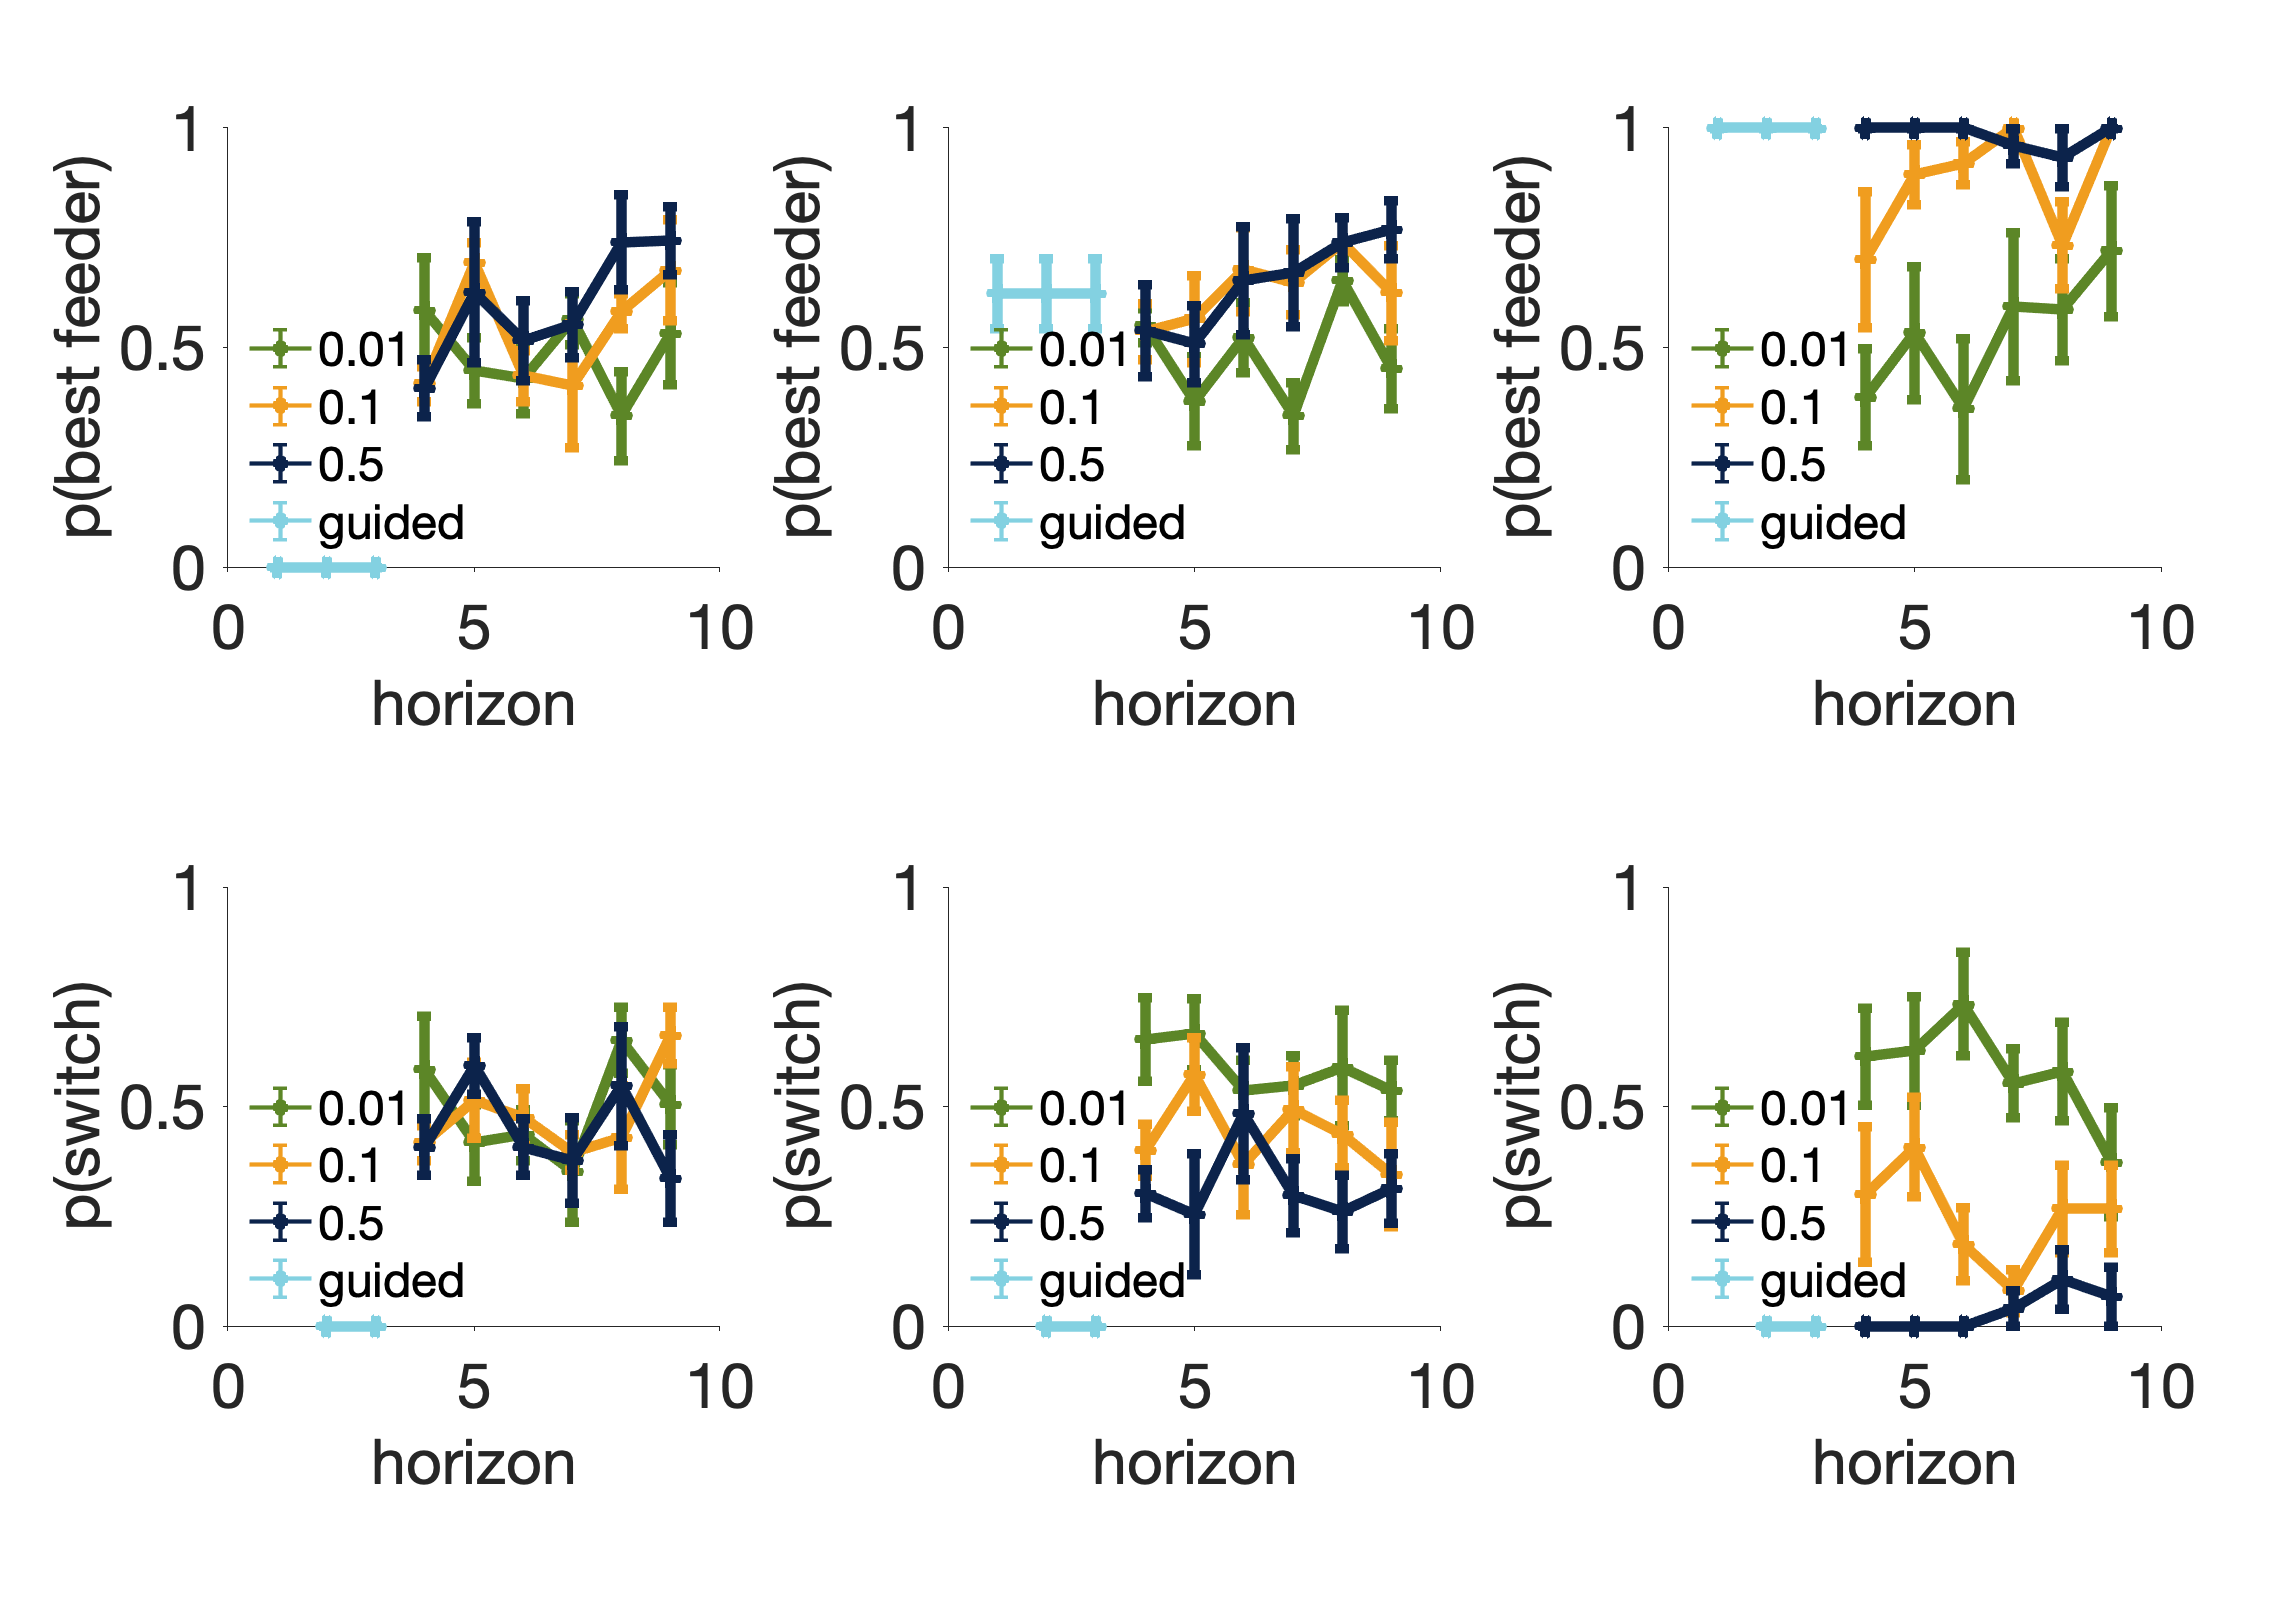
\includegraphics[width=0.8\textwidth]{../Figs/modelA.png}
		\end{center}
\end{figure}
\subsubsection{model B}
 \begin{figure}[H]
		\begin{center}
			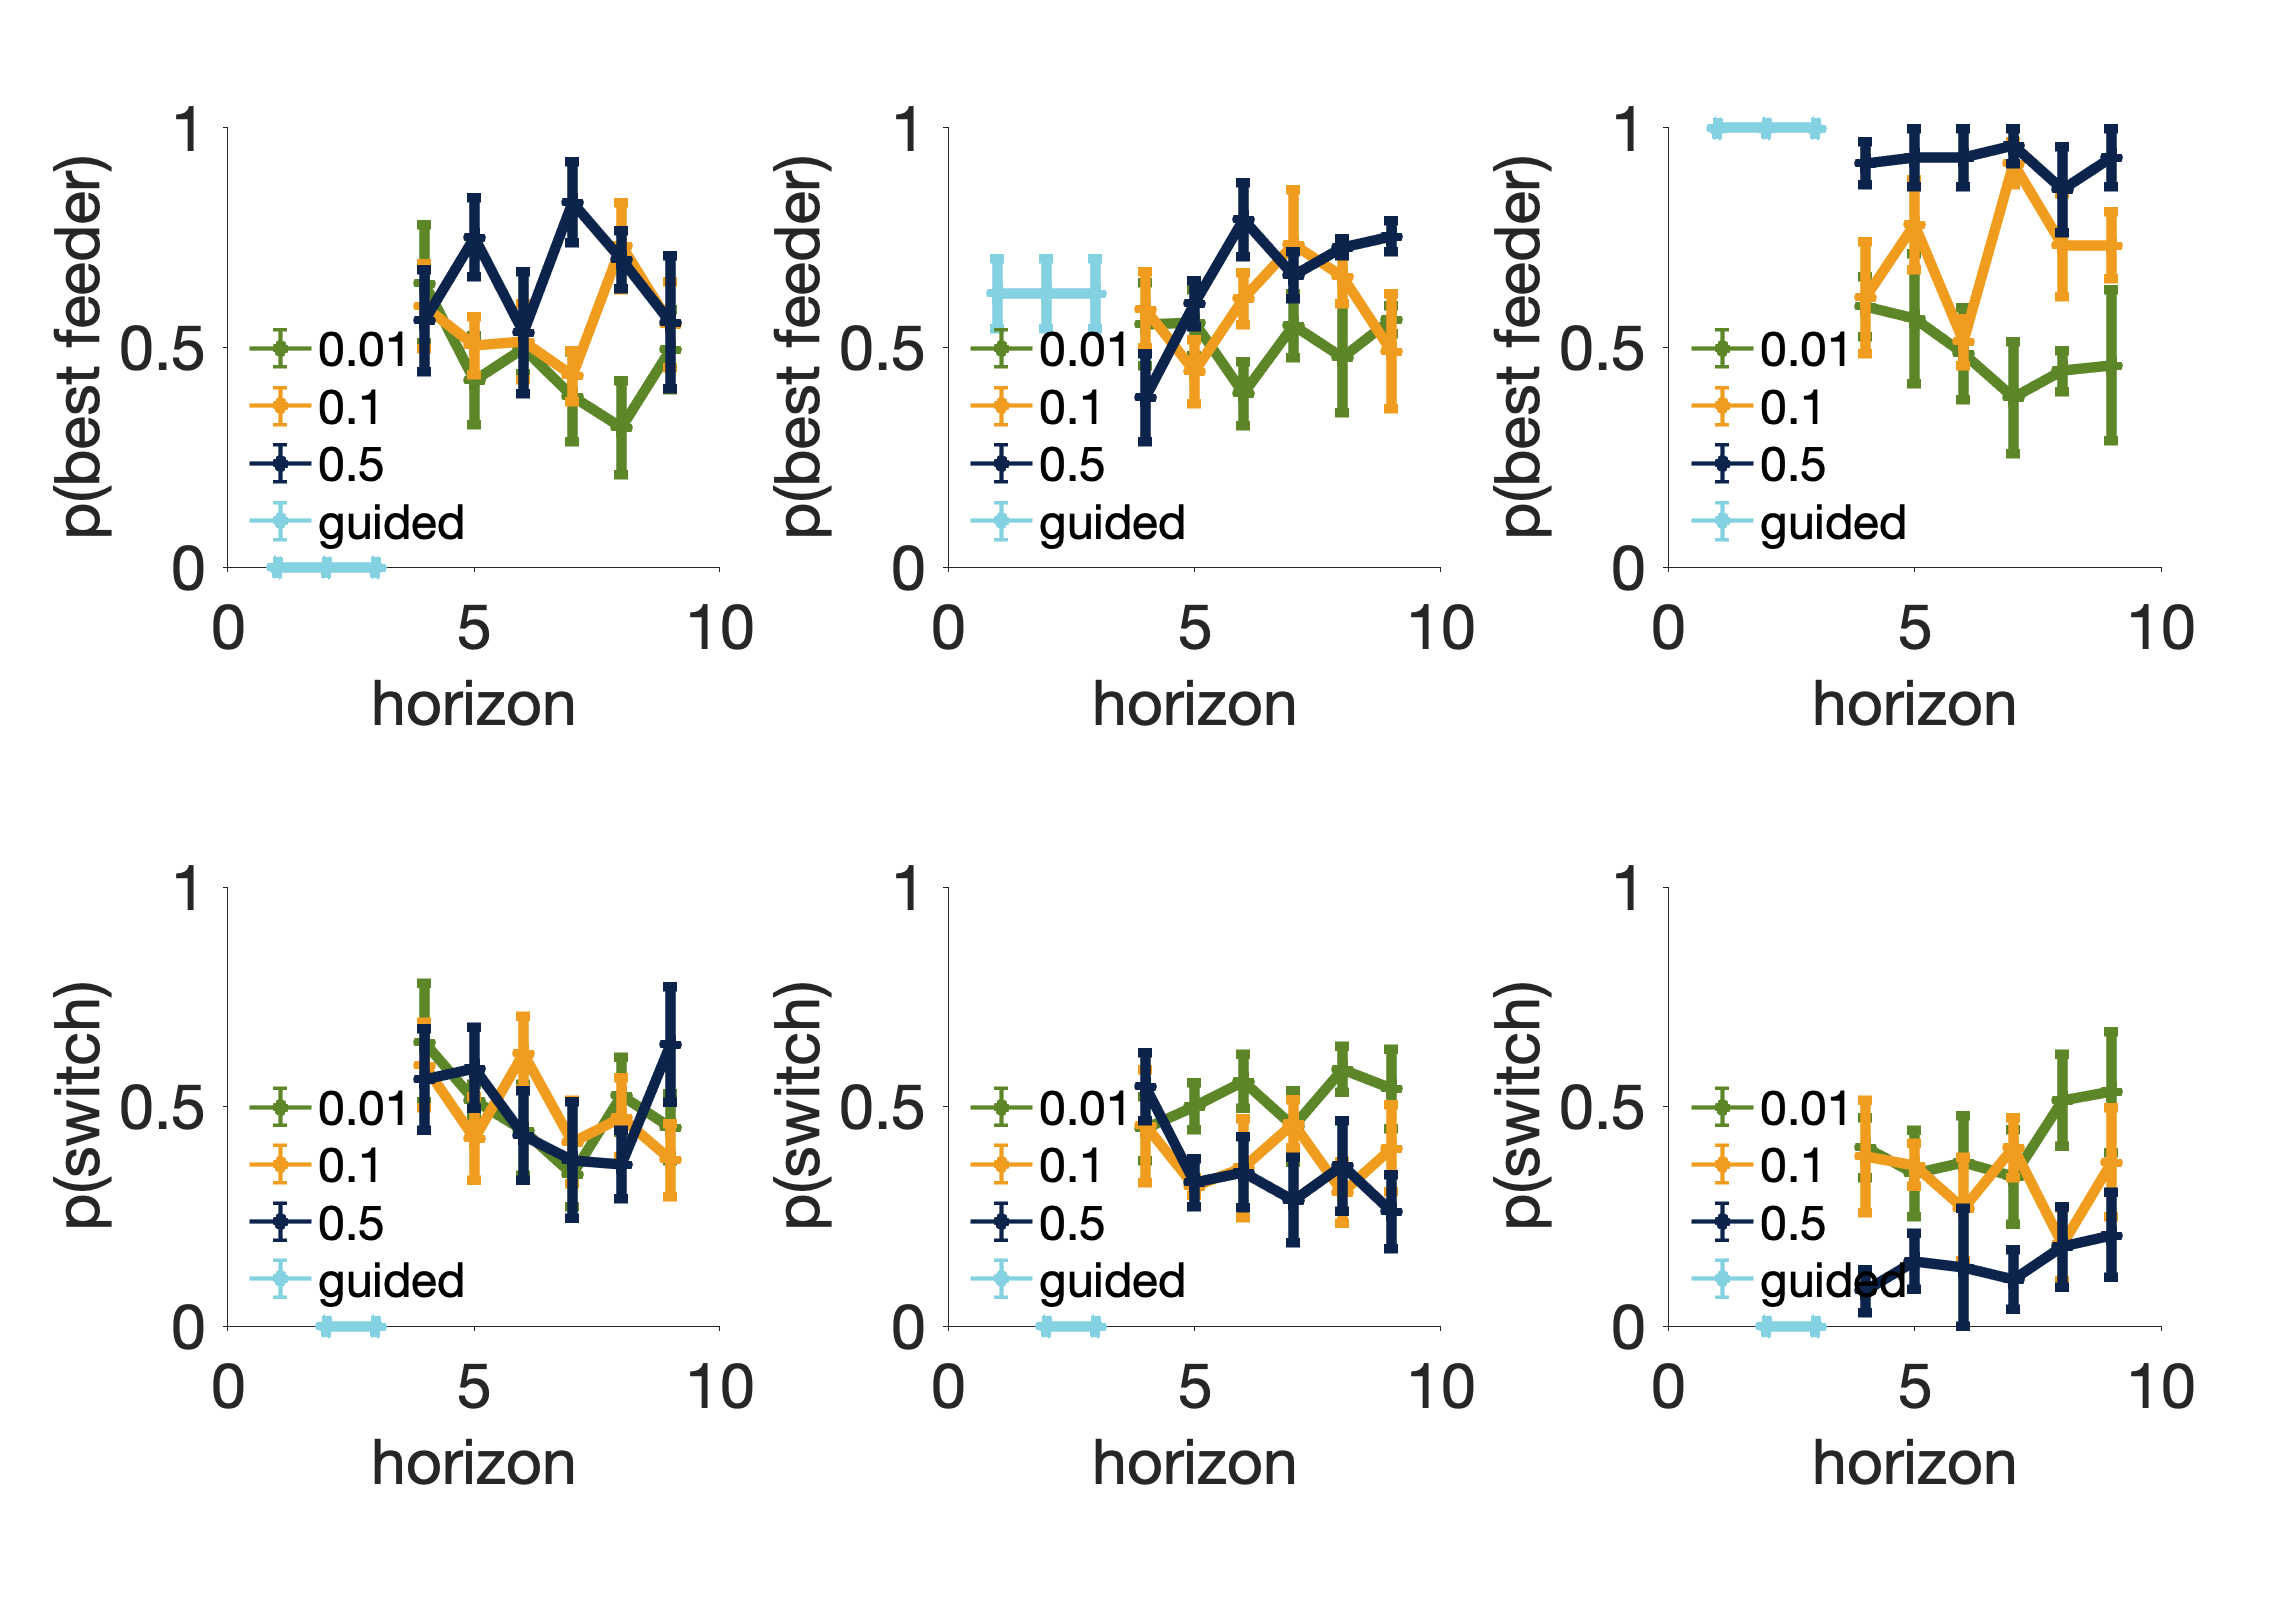
\includegraphics[width=0.85\textwidth]{../Figs/modelB.png}
		\end{center}
\end{figure}
\subsubsection{model C}
 \begin{figure}[H]
		\begin{center}
			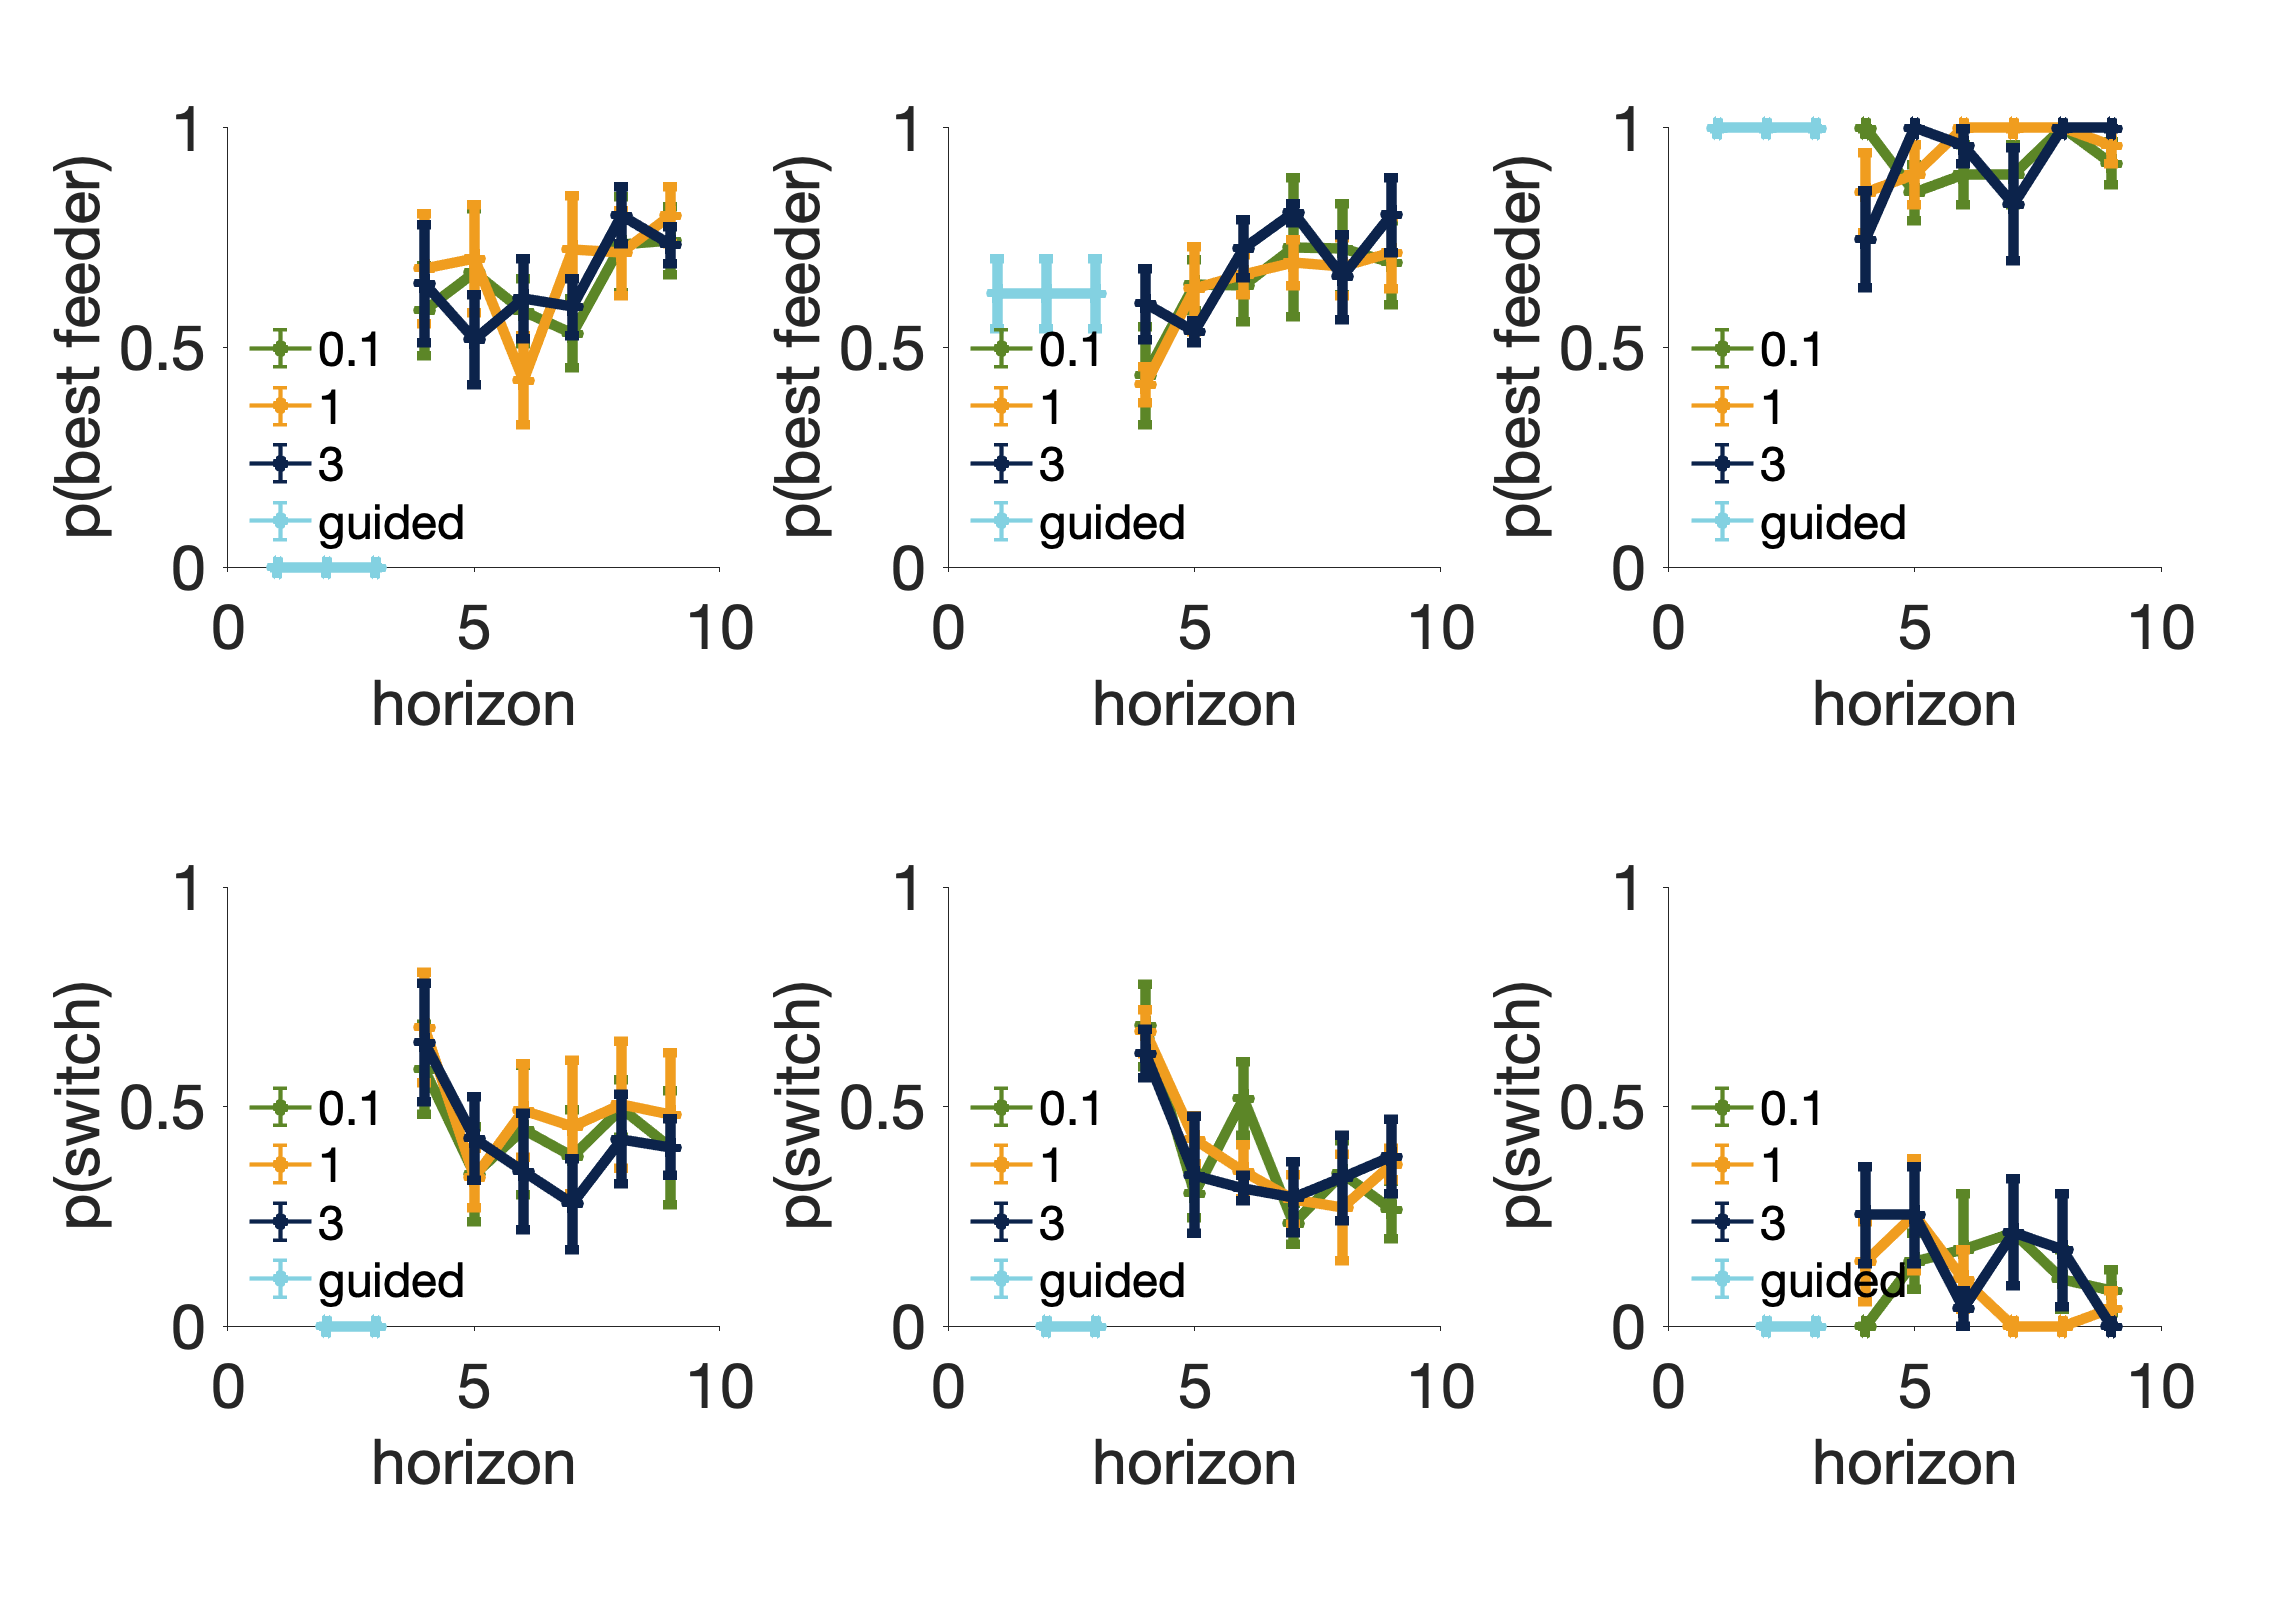
\includegraphics[width=0.85\textwidth]{../Figs/modelC.png}
		\end{center}
\end{figure}
\subsubsection{model D}
 \begin{figure}[H]
		\begin{center}
			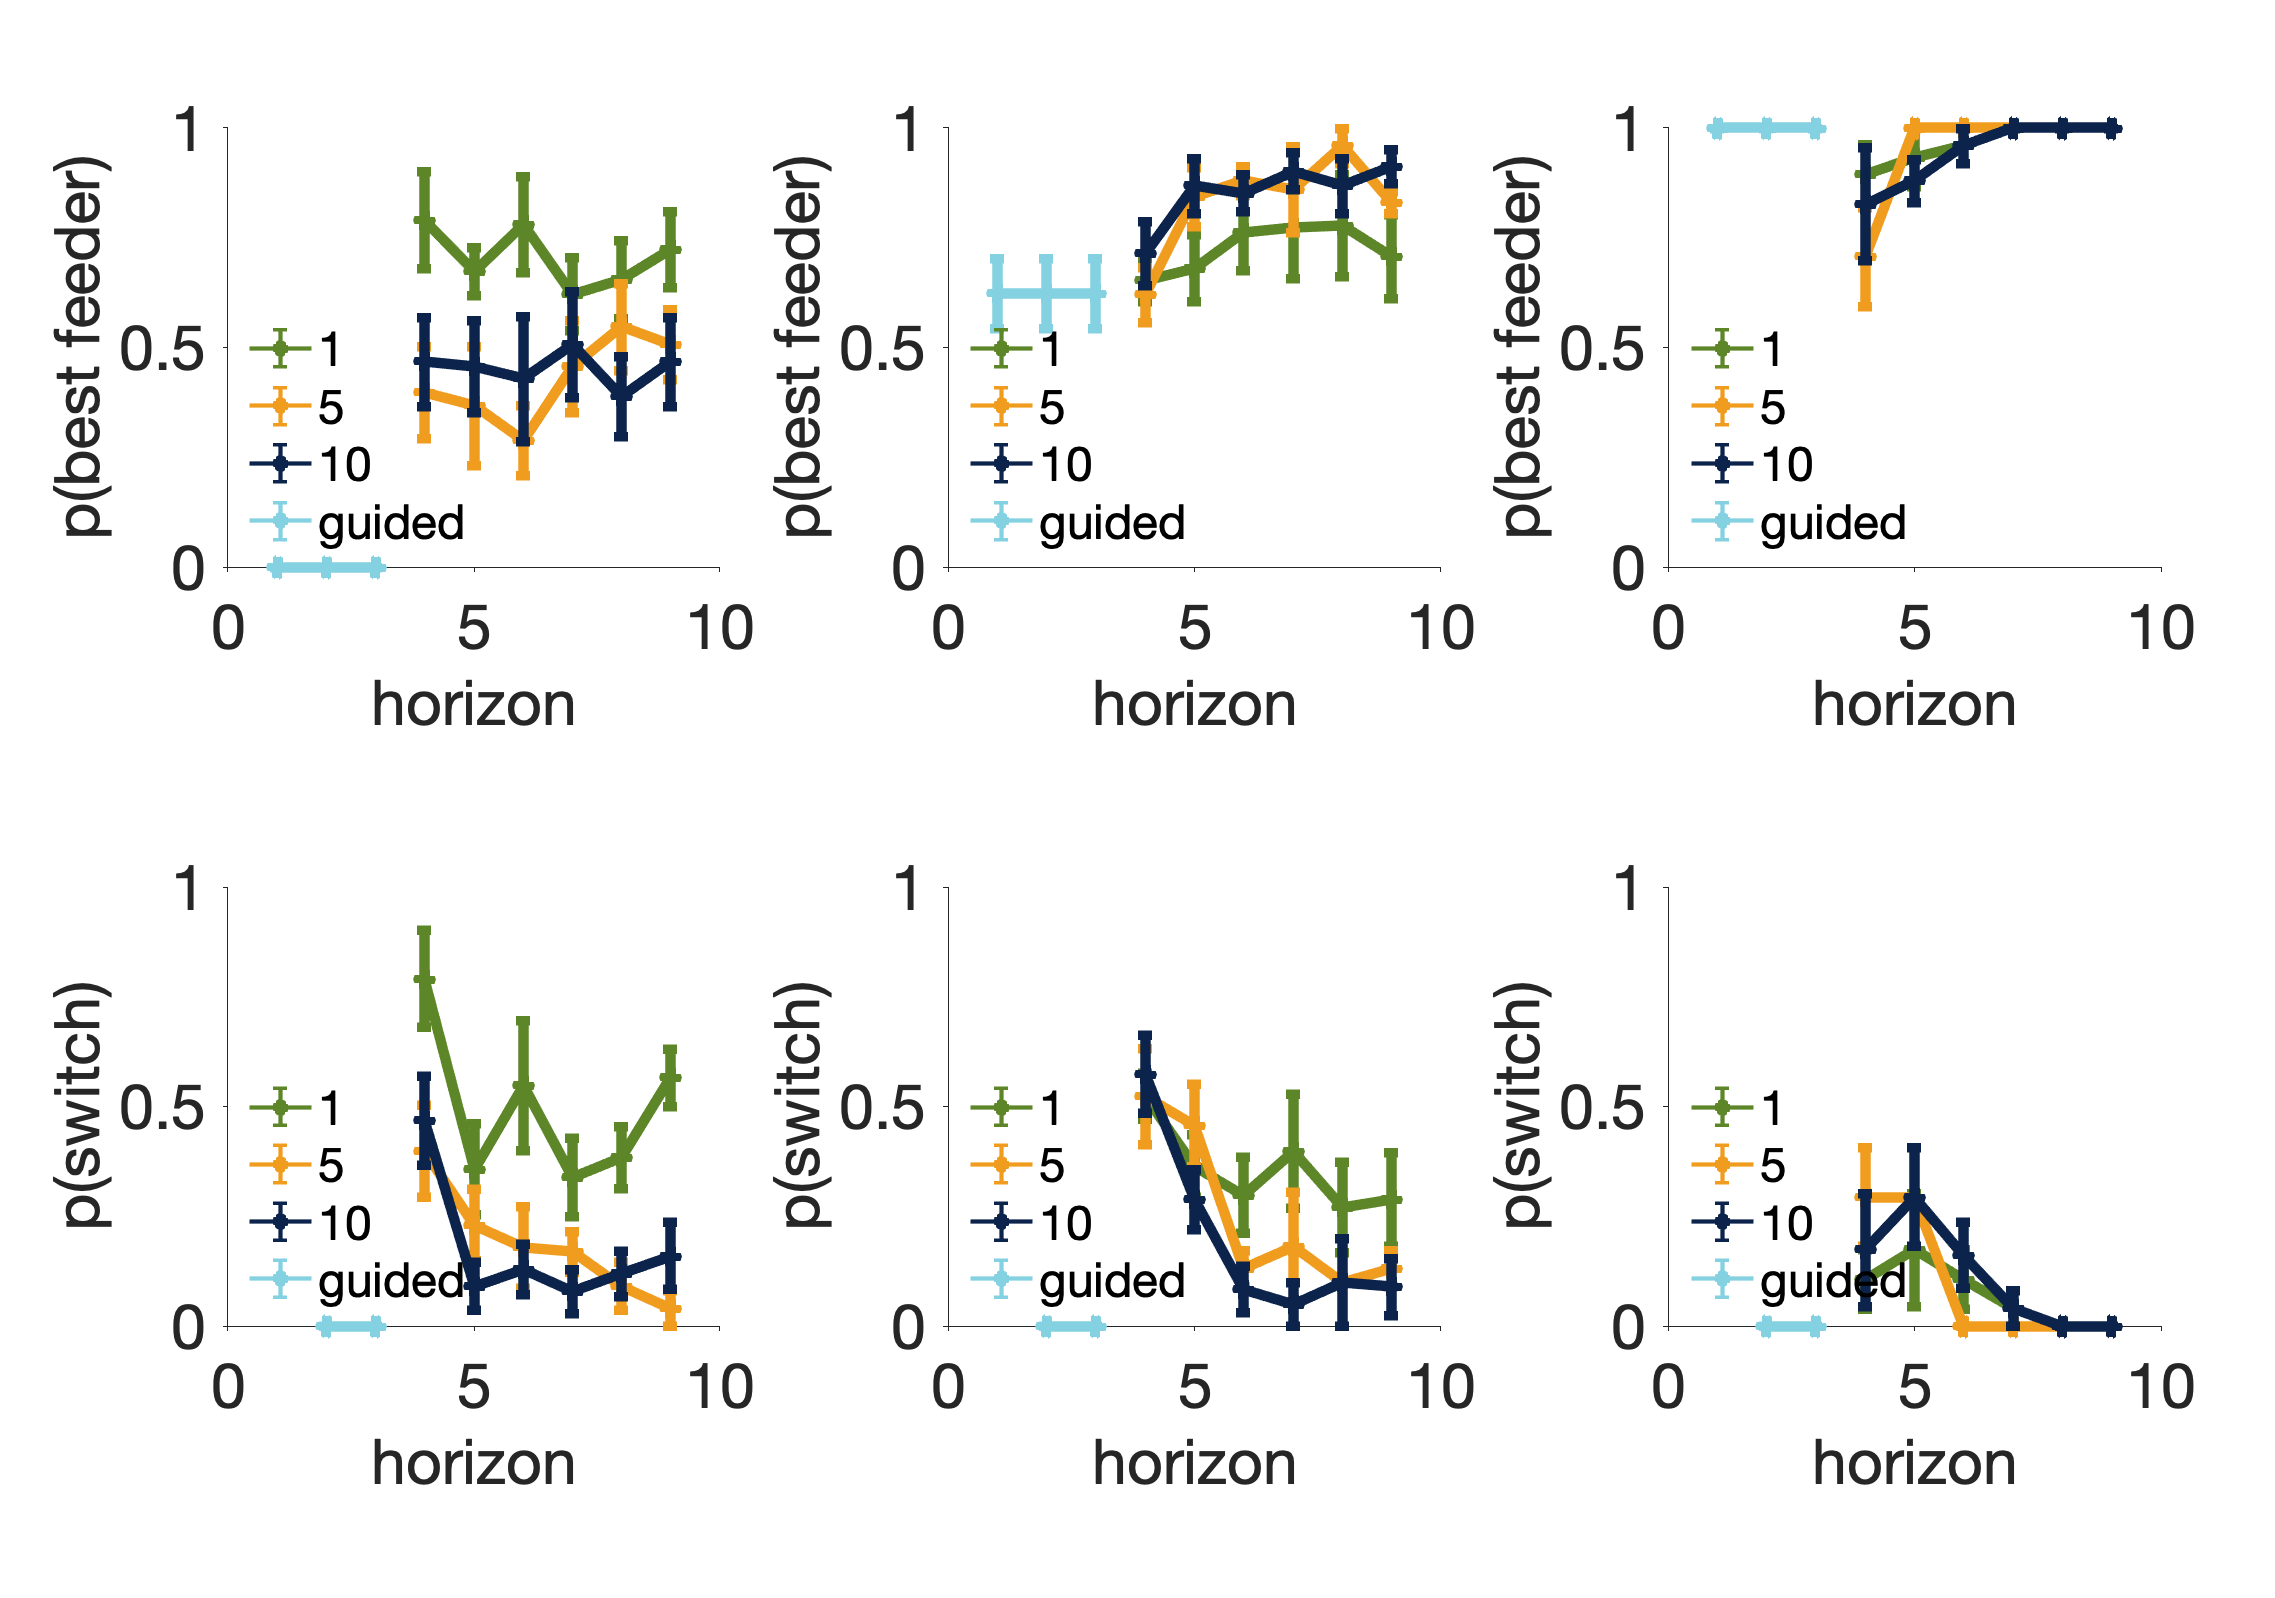
\includegraphics[width=0.85\textwidth]{../Figs/modelD.png}
		\end{center}
\end{figure}
 
\end{document}

